\documentclass[10pt]{beamer}

\usetheme[progressbar=frametitle]{metropolis}
\usepackage{appendixnumberbeamer}

\usepackage{booktabs}
\usepackage[scale=2]{ccicons}

\usepackage{pgfplots}
\usepgfplotslibrary{dateplot}

\usepackage{xspace}
\newcommand{\themename}{\textbf{\textsc{metropolis}}\xspace}

\usepackage[english]{babel}
\usepackage{tikz}
\usepackage{pgfplots}
\usepackage{caption}
\usepackage{circuitikz}
\usepackage{listings}
\usepackage{pgfplotsthemetol}
\captionsetup{justification=centering}
\usetikzlibrary{plotmarks}
\usepackage[utf8]{inputenc}
\usepackage[english]{babel}
\usepackage{amsmath}
\usepackage{amsfonts}
\usepackage{amssymb}
\usepackage{graphicx}
\usepackage{setspace}
\usepackage{parskip}
\usepackage{amsthm}
\usepackage{fancyhdr}
\usepackage{booktabs}
\usepackage{hyperref}
\usepackage{pgfplots}% This uses tikz
\pgfplotsset{compat=newest}% use newest version
\usepackage{sidecap}
\usepackage{tikz}
\usepackage{tikz-3dplot}
\usepackage{xcolor}
\usepackage{xstring}
\usepackage{multirow}
\usepackage{adjustbox}

\usepackage{caption}
\usepackage{color}
\usepackage{array}
\usepackage{wrapfig}
\usepackage{listings}
\captionsetup{justification=centering}
\usetikzlibrary{plotmarks}

\usepackage{media9}%
\usepackage{hyperref}

\usepackage[scale=2]{ccicons}
\usepackage{minted}

\usemintedstyle{trac}

\title{SCELP: Low delay audio coding with noise shaping based on spherical vector quantization}
\subtitle{Coding of Audiovisual Contents}
\date{Barcelona, \today}
\author{Miquel Oller Oliveras, Alvaro Scherk Fontanals}
\institute{ \vspace{40pt} 
\includegraphics[width=85pt]{./img/logoUPC.png}\hspace{200pt}
\includegraphics[width=30pt]{./img/logo-etsetb.png}}
\definecolor{mDarkTeal}{HTML}{23373b}
\setbeamercolor{section page}{bg=mDarkTeal}




\begin{document}

\maketitle

\begin{frame}{Table of Contents:}
  \tableofcontents
\end{frame}



\begingroup
\setbeamercolor{section title}{fg=white}
\setbeamercolor{background canvas}{bg=mDarkTeal}
\section{Pràctica 1: Tècniques de Mesura}
\endgroup

\begin{frame}{Objectius}
  \begin{itemize}
    \item Aprendre a mesurar pressions i velocitats en un fluid
    \item Calcular pèrdues de càrrega lineals i singulars
    \item Estudiar com varien les línies de càrrega i piezomètriques d'un Venturi
  \end{itemize}
\end{frame}
\begin{frame}{Elements de mesura}
  \begin{itemize}
    \item Tub piezomètric: \hspace{0.1\linewidth}
      \includegraphics[width=0.3\linewidth]{./img/P1/Piezo.PNG}\\
    \item Manòmetre líquid de columna inclinada: \hspace{0.05\linewidth}
    \includegraphics[width=0.3\linewidth]{./img/P1/columna.PNG}
    \item Manòmetre metàl·lic:\hspace{0.1\linewidth}
    \includegraphics[width=0.2\linewidth]{./img/P1/manMet}
    \item Transductor de pressió:\hspace{0.1\lineswidth}
    \includegraphics[width=0.3\linewidth]{./img/P1/trsPress}
  \end{itemize}
\end{frame}
\begin{frame}{Elements de mesura}
  \begin{itemize}
    \item Sonda de Prandtl:\\
      \includegraphics[width=0.55\linewidth]{./img/P1/prand2.PNG}\hspace{0.07\linewidth}
      \includegraphics[width=0.3\linewidth]{./img/P1/Prandtl.PNG}
      \begin{equation*}
        \frac{P_2}{\gamma} + z_2 + \frac{c_2 ^2}{2g} =\frac{P_3}{\gamma} + z_3 + \frac{c_3 ^2}{2g} + \Delta h_{23}
      \end{equation*}
      \begin{equation*}
        \Delta z = 0 \hspace{1.2cm} c_3 = 0\hspace{1.2cm} \Delta h_{23} = 0
      \end{equation*}
      \begin{equation*}
        c_2 = c = \sqrt[]{2\cdot g \cdot \frac{\Delta P}{\gamma}}
      \end{equation*}
      \begin{equation*}
        c\hbox{[m/s]} \cong 4\cdot \sqrt[]{(h_b - h_a)[{mm}_cH_2O]}
      \end{equation*}
  \end{itemize}
\end{frame}

\begin{frame}{Pèrdues de càrrega}
  \includegraphics[width=\linewidth]{./img/P1/perdues}
\end{frame}

\begin{frame}{Pèrdues de càrrega lineals}
    \begin{center}\includegraphics[width=0.3\linewidth]{./img/P1/tub12}\end{center}\\
    Dades:\begin{table}[h!]
    \centering
      \begin{tabular}{|c|c|c|}
        \hline L $[m]$ & D $[m]$ & \Delta z $[m]$\\ [2pt]
        \hline 0,8 & 0,026 & 0 \\ [2 pt]
        \hline
      \end{tabular}
    \end{table}

    Mesures:$$\frac{P_1 - P_2}{\gamma} = 6,5\, mm_c H_2O = 5,417\, m_cAire$$
    $$Q = 19\,\frac{\hbox{m}^3}{\hbox{h}} = \frac{19}{3600} = \,\frac{\hbox{m}^3}{\hbox{s}}\hspace{1.5cm} c = \frac{Q}{A} = \frac{19}{3600\cdot \frac{\pi\cdot 0,026^2}{4}} = 9,94\,\frac{\hbox{m}}{\hbox{s}}$$
\end{frame}
\begin{frame}{Pèrdues de càrrega lineals}
    Per {\it Bernoulli}:
    $$\frac{P_1}{\gamma} + z_1 + \frac{c_1 ^2}{2g} =\frac{P_2}{\gamma} + z_2 + \frac{c_2 ^2}{2g} + \Delta h_{12} $$
    Pel tram lineal $z_1 = z_2$, $D$ constant $\rightarrow$ $c$ constant:
    $$\frac{P_1 - P_2}{\gamma} = \Delta h_{12}$$
    Per {\it Darcy - Weisbach}:
    \begin{equation*}
      \Delta h = \lambda \cdot \frac{L}{D} \cdot \frac{c^2}{2g} = \frac{P_1 - P_2}{\gamma}
    \end{equation*}
    \begin{equation*}
      \lambda = \frac{2\cdot D \cdot \frac{P_1 - P_2}{\gamma}}{L\cdot c^2} = \frac{2\cdot 0,026 \cdot 5,417}{0,8 \cdot 9,94^2} = 0,00356
    \end{equation*}
\end{frame}

\begin{frame}{Pèrdues de càrrega singulars}
  \centering\includegraphics[width=0.3\linewidth]{./img/P1/tub48}\\
Mesures en $m_{cAire}$,
\begin{table}[h!]
\centering
\begin{tabular}{|c|c|c|c|}
\hline Colze & $\frac{P_1-P_2}{\gamma}$ [$m_{cAire}$]& $\Delta z$ [m]& $\Delta h_{tot}$[$m_{cAire}$]\\ [2pt]
\hline 180º & 2,083 & 0,08 & 2,003 \\ [2 pt]
\hline 135º & 0,833 & 0,09 & 0,743 \\ [2 pt]
\hline 90º & 2,083 & 0,145 & 1,938 \\ [2 pt]
\hline
\end{tabular}
\end{table}
\end{frame}

\begin{frame}{Pèrdues de càrrega singulars}
$$\frac{P_1}{\gamma} + z_1 + \frac{c_1 ^2}{2g} =\frac{P_2}{\gamma} + z_2 + \frac{c_2 ^2}{2g} + \Delta h_{12}  + \Delta h_s$$
$D = cte \rightarrow c = cte, $i considerant $h_{tot} = h_{12} + h_s$,
$$\frac{P_1}{\gamma} + z_1  =\frac{P_2}{\gamma} + z_2  + \Delta h_{tot} \hspace{0.8cm} \longrightarrow \hspace{0.8cm} \Delta h_{tot} = \frac{P_1 - P_2}{\gamma} -\Delta z$$
$$\Delta h_s = \Delta h_{tot} - \Delta h_{l} \hspace{1.2cm} K = \frac{2\cdot g \cdot \Delta h_s}{c^2}$$

Tenim una bifurcació, mesurem velocitat amb sonda Prantdl,
$$c\hbox{[m/s]} \cong 4\cdot \sqrt[]{(h_b - h_a)[mm_cH_2O]}$$
\end{frame}

\begin{frame}{Pèrdues de càrrega singulars}
  \begin{table}[h!]
    \centering
    \begin{adjustbox}{max width=1.05\textwidth}
    \begin{tabular}{|c|c|c|c|c|c|c|c|c|}
      \hline Colze & $\Delta h_{tot}$ [mcAire] & $h_b-h_a$ [mmcAigua] & $c$ [m/s]& $L$ [m] & $D$ [m]& $\Delta h_l$ [mcAire]& $\Delta h_S$ [mcAire]& $K$ \\ [2pt]
      \hline 180º & 2,003 & 2 & 5,66 & 0,2 & 0,026 & 0,0447 & 1,9583 & 1,199 \\
      \hline 135º & 0,743 & 2 & 5,66 & 0,2 & 0,026 & 0,0447 & 0,698 & 0,428 \\
      \hline 90º & 1,938 & 3 & 6,93 & 0,2 & 0,026 & 0,067 & 1,871 & 0,764 \\\hline
    \end{tabular}
  \end{adjustbox}
  \end{table}
\vspace{1cm}
Tal i com era d'esperar, $K_{180º} \geq K_{90º} \geq K_{135º}$.

\end{frame}

\begin{frame}{Venturi}
  \includegraphics[width=\linewidth]{./img/P1/p2v.PNG}
\end{frame}
\begin{frame}{Venturi}
  Sonda Prantdl,
$$\Delta h = 9 mm_cH_2O \rightarrow c_A = 12 \frac{m}{s}$$
$$D_A = 70 cm \hspace{1.2cm}\rightarrow \hspace{1.2cm} Q = 12 \cdot \frac{\pi \cdot 0.07^2}{4} = 0,0462 \frac{m^3}{s}$$

\begin{table}[h!]
\centering
\begin{tabular}{|c|c|c|c|}
\hline
Punt & 1 & 5 & 8 \\ [2pt]
\hline
$\frac{\Delta P}{\gamma}$ [$mm_cH2O$] & 30 & -85 & 15 \\ [2 pt]
\hline
\end{tabular}
\end{table}

\end{frame}

\begin{frame}{Venturi}

$$\hbox{Cota piezomètrica} = \frac{P}{\gamma} + z = \frac{P}{\gamma} $$
$$ \hbox{Cota de càrrega} = \frac{P}{\gamma} + z + \frac{c^2}{2g} = \frac{P}{\gamma} + \frac{c^2}{2g}$$
$$c = \frac{Q}{A} = \frac{Q}{\frac{\pi \cdot D^2}{4}}$$
\begin{table}[h!]
\centering
\begin{tabular}{|c|c|c|c|}
\hline
Punt & 1 & 5 & 8 \\ [2pt]
\hline
$D$ [mm] & 95,8&38,7&89,8\\[2pt]
\hline
$c$ [m/s]& 6,407&39,260 & 7,2916\\[2pt]
\hline
$\frac{ P}{\gamma}$ [mcAire] & 25 & -70,83 & 12,5 \\ [2pt]
\hline
Piezomètrica & 25& -70,83 & 12,5\\[2pt]
\hline
Càrrega & 27,09 &&15,21\\[2pt]
\hline
\end{tabular}

\end{table}
\end{frame}

\begin{frame}{Venturi}
  \centering
  \includegraphics[width=\linewidth]{./img/P1/Linies}
\end{frame}













\begingroup
\setbeamercolor{section title}{fg=white}
\setbeamercolor{background canvas}{bg=mDarkTeal}
\section{Pràctica 2: Simulació Fluidodinàmica}
\endgroup

  \begin{frame}{Repàs Teòric}
    \centering
    \includegraphics[width=\linewidth]{./img/P3/teoCL.PNG}
  \end{frame}

  \begin{frame}{Desprendiment de la Capa Límit }
    \centering
    \includegraphics[width=\linewidth]{./img/P3/2.PNG}
  \end{frame}

  \begin{frame}{Desprendiment de la Capa Límit }
    \centering
    \includegraphics[width=\linewidth]{./img/P3/3.PNG}
  \end{frame}

  \begin{frame}{Visualització de la capa límit}
    \centering
    \includegraphics[width=\linewidth]{./img/P3/capa_limit.PNG}
  \end{frame}
  \begin{frame}{Visualització de la capa límit: Perfil de velocitats}
    \centering
    \includegraphics[width=\linewidth]{./img/P3/capa_limit2.PNG}
  \end{frame}
  \begin{frame}{Visualització de la capa límit: Perfil de velocitats}
    \centering
    \includegraphics[width=\linewidth]{./img/P3/capa_limit3.PNG}
  \end{frame}
  \begin{frame}{Visualització del les línies de corrent}
    \centering
    \includegraphics[width=\linewidth]{./img/P3/stream_function.PNG}
  \end{frame}
  \begin{frame}{Visualització del les línies de corrent}
    \centering
    \includegraphics[width=\linewidth]{./img/P3/stream_function2.PNG}
  \end{frame}
  \begin{frame}{Visualització de les pressions}
    \centering
    \includegraphics[width=\linewidth]{./img/P3/presins.PNG}
  \end{frame}








  \begingroup
  \setbeamercolor{section title}{fg=white}
  \setbeamercolor{background canvas}{bg=mDarkTeal}
  \section{Pràctica 3: Anàlisi Simulatori}
  \endgroup

  \begin{frame}{Visualització de la velocitat $0^{\circ}$}
    \centering
    \includegraphics[width=\linewidth]{./img/P4/v0.PNG}
  \end{frame}
  \begin{frame}{Visualització de la velocitat $0^{\circ}$}
    \centering
    \includegraphics[width=\linewidth]{./img/P4/v00.PNG}
  \end{frame}
  \begin{frame}{Visualització de la velocitat $0^{\circ}$}
    \centering
    \includegraphics[width=\linewidth]{./img/P4/v000.PNG}
  \end{frame}
  \begin{frame}{Visualització de la pressió $0^{\circ}$}
    \centering
    \includegraphics[width=\linewidth]{./img/P4/p0.PNG}
  \end{frame}

  \begin{frame}{Visualització de la velocitat $5^{\circ}$}
    \centering
    \includegraphics[width=\linewidth]{./img/P4/v5.PNG}
  \end{frame}
  \begin{frame}{Visualització de la velocitat $5^{\circ}$}
    \centering
    \includegraphics[width=\linewidth]{./img/P4/v55.PNG}
  \end{frame}
  \begin{frame}{Visualització de la velocitat $5^{\circ}$}
    \centering
    \includegraphics[width=\linewidth]{./img/P4/v555.PNG}
  \end{frame}
  \begin{frame}{Visualització de la pressió $5^{\circ}$}
    \centering
    \includegraphics[width=\linewidth]{./img/P4/p5.PNG}
  \end{frame}

  \begin{frame}{Visualització de la velocitat $10^{\circ}$}
    \centering
    \includegraphics[width=\linewidth]{./img/P4/v10.PNG}
  \end{frame}
  \begin{frame}{Visualització de la velocitat $10^{\circ}$}
    \centering
    \includegraphics[width=\linewidth]{./img/P4/v1010.PNG}
  \end{frame}
  \begin{frame}{Visualització de la velocitat $10^{\circ}$}
    \centering
    \includegraphics[width=\linewidth]{./img/P4/v101010.PNG}
  \end{frame}
  \begin{frame}{Visualització de la pressió $10^{\circ}$}
    \centering
    \includegraphics[width=\linewidth]{./img/P4/p10.PNG}
  \end{frame}

  \begin{frame}{Visualització de la velocitat $15^{\circ}$}
    \centering
    \includegraphics[width=\linewidth]{./img/P4/v15.PNG}
  \end{frame}
  \begin{frame}{Visualització de la velocitat $15^{\circ}$}
    \centering
    \includegraphics[width=\linewidth]{./img/P4/v1515.PNG}
  \end{frame}
  \begin{frame}{Visualització de la velocitat $15^{\circ}$}
    \centering
    \includegraphics[width=\linewidth]{./img/P4/v151515.PNG}
  \end{frame}
  \begin{frame}{Visualització de la velocitat $15^{\circ}$}
    \centering
    \includegraphics[width=\linewidth]{./img/P4/v15151515.PNG}
  \end{frame}
  \begin{frame}{Visualització de la pressió $15^{\circ}$}
    \centering
    \includegraphics[width=\linewidth]{./img/P4/p15.PNG}
  \end{frame}

  \begin{frame}{Visualització de la velocitat $18^{\circ}$}
    \centering
    \includegraphics[width=\linewidth]{./img/P4/v18.PNG}
  \end{frame}
  \begin{frame}{Visualització de la velocitat $18^{\circ}$}
    \centering
    \includegraphics[width=\linewidth]{./img/P4/v1818.PNG}
  \end{frame}
  \begin{frame}{Visualització de la velocitat $18^{\circ}$}
    \centering
    \includegraphics[width=\linewidth]{./img/P4/v181818.PNG}
  \end{frame}
  \begin{frame}{Visualització de la velocitat $18^{\circ}$}
    \centering
    \includegraphics[width=\linewidth]{./img/P4/v18181818.PNG}
  \end{frame}
  \begin{frame}{Visualització de la pressió $18^{\circ}$}
    \centering
    \includegraphics[width=\linewidth]{./img/P4/p18.PNG}
  \end{frame}



  \begin{frame}{Animació:}
      \vspace*{-70px}
      \hspace*{-30px}
      \includemedia[%
        width=1\linewidth,
        activate=pagevisible,%
        deactivate=pageclose,%
        addresource=./img/P4/P4_velocity_25graus.swf,%
        flashvars={%
          src=./img/P4/P4_velocity_25graus.swf % same path as in addresource!
          &autoPlay=true % default: false; if =true, automatically starts playback after activation (see option ‘activation)’
          &loop=true % if loop=true, media is played in a loop
          &controlBarAutoHideTimeout=0 %  time span before auto-hide
        }%
      ]{-}{./img/P4/P4_velocity_25graus.swf}%
  \end{frame}

  \begin{frame}{Gràfics coeficients: $c_L$}
    \centering
    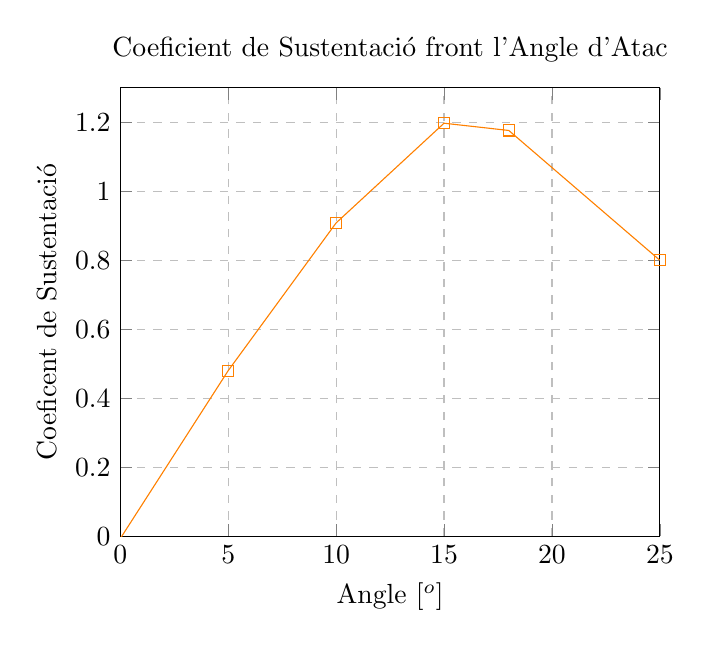
\begin{tikzpicture}
      \begin{axis}[
          title={Coeficient de Sustentació front l'Angle d'Atac},
          xlabel={Angle [$^o$]},
          ylabel={Coeficent de Sustentació},
          xmin=0, xmax=25,
          ymin=0, ymax=1.3,
          xtick={0,5,10,15,20,25},
          ytick={-0.1,0,0.2,0.4,0.6,0.8,1,1.2},
          ymajorgrids=true,
          xmajorgrids=true,
          grid style=dashed,
          ]
      \addplot[
        color=orange,
        mark=square,
        ]
        coordinates {
        (0,-0.007)(5,0.48)(10,0.9084)(15,1.1975)(18,1.1765)(25,0.8)
        };
      \end{axis}
    \end{tikzpicture}
  \end{frame}


  \begin{frame}{Gràfics coeficients: $c_D$}
    \centering
    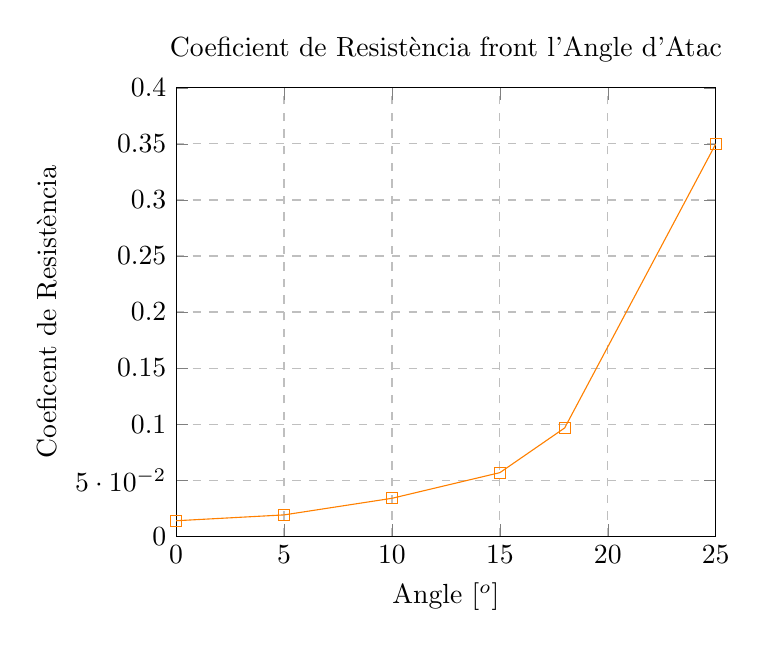
\begin{tikzpicture}
      \begin{axis}[
          title={Coeficient de Resistència front l'Angle d'Atac},
          xlabel={Angle [$^o$]},
          ylabel={Coeficent de Resistència},
          xmin=0, xmax=25,
          ymin=0, ymax=0.4,
          xtick={0,5,10,15,20,25},
          ytick={0,0.05,0.1,0.15,0.2,0.25,0.3,0.35,0.4},
          ymajorgrids=true,
          xmajorgrids=true,
          grid style=dashed,
          ]
      \addplot[
        color=orange,
        mark=square,
        ]
        coordinates {
        (0,0.013779)(5,0.019)(10,0.033807)(15,0.05671)(18,0.09658)(25,0.35)
        };
      \end{axis}
    \end{tikzpicture}
  \end{frame}


\maketitle

\end{document}
